% filepath: /home/mh19137/scale_morphology/paper/A_appendix_efa_area.tex

\documentclass[11pt,a4paper,notitlepage]{article}

\usepackage[utf8]{inputenc}
\usepackage{amsmath}
\usepackage{graphicx}
\usepackage{mathtools}
\usepackage{hyperref}
\usepackage{natbib}

\author{Richard Lane}
\title{
	Geometric Operations in Fourier Space: A Practical Guide to Elliptic Fourier Analysis for Morphology
}

\begin{document}

\maketitle

\begin{abstract}
	\begin{itemize}
		\item EFA is used by lots of different people, usually just for extracting features
		\item However, it is actually extremely powerful and nice - its a Fourier representation of shape!
		\item Which means it has all the information about shape - it isn't just a collection of features
		\item This means some things are easier in EFA space than in real space:
		      \begin{itemize}
			      \item Calculating area (not novel; appendix with maths)
			      \item Aligning two objects (not novel, but possibly an extension of existing stuff; appendix with maths)
			      \item Interpreting features - dimensionality-reduced (PCA, LDA) features can have intuitive geometrical interpretations (i think novel)
		      \end{itemize}
		\item TODO - probably should illustrate the above with fish scales
		\item Thinking about EFA as a complete Fourier representation of shapes gives us geometric intuition about why the above things work -
		      rethinking EFA in this way is valuable for morphology studies because intuition is important.
		\item Working + easily runnable code is provided for all the above examples, which is useful
		\item This is an under-appreciated aspect of EFA, awareness of which could enable more powerful and interpretable analyses of shapes
	\end{itemize}
\end{abstract}

\section{Introduction}
Elliptic Fourier Analysis (EFA) has been an important technique in quantitative shape analysis
since Zahn \& Roskies~\cite{Zahn1972} in 1972 and subsequently Kuhl and Giardina~\cite{Kuhl1982}.
It has been widely used in biology to describe the outlines of cells, organs, and
organisms~\cite{Iwata2002,GAYO2023739948,Diaz1989,Jeong2007,Chitwood_Otoni_2017} and is often used
in downstream processing for
PCA~\cite{VifaraVega2025,Paige2025,SLEZAK2020107102},
LDA~\cite{Chitwood_Otoni_2017},
or classification~\cite{Ghanem2025}.

Recent efforts have been made to popularise and explain the intuition and utility of EFA to varied
audiences in many fields~\cite{Caple2017,Courtenay2022,wu2024reliable}.
A review of EFA in the biomedical sciences found that EFA is a valuable tool for
feature extraction, classification and shape modelling~\cite{Valizadeh2022}.
However, these Fourier coefficients are not merely descriptive features; they form a conjugate space to
the original outline, containing the full geometric information of the shape. As in classical 1-dimensional signal processing,
certain operations that are complex in the spatial domain are greatly simplified in the Fourier domain.
Here, we illustrate the utility of working in EFA-space with geometric examples, and provide intuitive geometric insights
into why this should be expected given the properties of the EFA expansion.

Previous work~\cite{Sjostrand_Ericsson_Larsen_2006} has shown that closed-form expressions in terms of EFA coefficients
exist for finding the area and centre of gravity and for performing ordinary Procrustes analysis~\cite{Gower2004}.
Expressions for these are re-derived here from first principles and intuitive geometrical explanations provided.
Examples of the alignment procedure are provided and eigenshapes produced for the objects in the fashion-MNIST~\cite{} dataset
to illustrate the utility of working in EFA space.
In addition, a novel solution is proposed previously unaddressed assumption in~\cite{Sjostrand_Ericsson_Larsen_2006} that,
when aligning two objects, there is correspondence between the EFA parameterisation of the two objects.
Complete and trivially runnable code is provided for all the examples given.


\section{Elliptic Fourier Analysis}
\subsection{Definition}
\label{app:efa-definition}
Any closed 2D contour $\left(x(t), y(t)\right)$ can be approximated as a sum over harmonic orders;
as a function of the parameter $t$, periodic over $\left[0, 2\pi \right]$:
\begin{equation}
	\label{eqn:EFDs}
	\begin{aligned}
		x(t) & = a_0 + \sum_{n=1}^{N}
		\left(
		a_n\cos(nt) + b_n\sin(nt)
		\right)                       \\
		y(t) & = c_0 + \sum_{n=1}^{N}
		\left(
		c_n\cos(nt) + d_n\sin(nt)
		\right)
	\end{aligned}
\end{equation}
which allows us to encode a shape as an $\left(N\times4\right)$ list of coefficients $\left\{a_n,b_n,c_n,d_n\right\}$.

An example showing the reconstruction of a shape from equally-spaced points on its perimeter up to various orders
can be seen in Figure~\ref{fig:efa_example}.
\begin{figure}[h!]
	\centering
	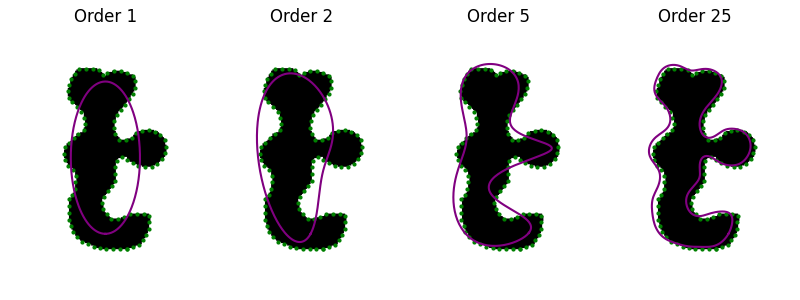
\includegraphics[width=\textwidth]{blob_efa.png}
	\caption{
		An illustration of an EFA reconstruction.
		Harmonics of progressively higher order are added to resolve finer details around the shape.
		Points (green) are found around the original object (black), and the EFA series (purple) is fit to them.
	}
	\label{fig:efa_example}
\end{figure}

The coefficients $a_0$ and $c_0$ set the location of the shape.
Since the contour is a periodic function of $t$, phase shifting the Fourier components transforms
the contour by moving its start point but leaving its shape unchanged.
Therefore, we have a choice of phase convention -- we are free to choose the starting point of the contour, without
having an effect on its shape.

\subsection{Finding the Area in Fourier Space}
We will start from Green's theorem in the plane. For any vector field $\vec{v}$ and closed contour $C$:
\begin{equation}
	\label{eqn:green_theorem}
	\oint_C \vec{v} \cdot d\vec{l} = \iint_D (\nabla \times \vec{v}) \cdot d\vec{A}
\end{equation}
If we choose $\vec{v} = \frac{1}{2}\left(-y, x\right)$, we find that the curl on the RHS evaluates to 1.

This gives us the area $A$:
\begin{equation}
	\label{eqn:area_int}
	A = \frac{1}{2}\oint_C \left(-y, x\right) \cdot \left(dx, dy\right)
\end{equation}
However, for a curve $C$ described by our EFDs we know $x$ and $y$ from Eq.~\ref{eqn:EFDs},
and can write down expressions for the line elements $dx = \frac{dx}{dt}dt$ and $dy = \frac{dy}{dt}dt$
in terms of the parameter $t$:

\begin{equation}
	\label{eqn:EFDs_derivative}
	\begin{aligned}
		dx & = dt\sum_{n=1}^{N}
		n\left(
		-a_n\sin(nt) + b_n\cos(nt)
		\right)                 \\
		dy & = dy\sum_{n=1}^{N}
		n\left(
		-c_n\sin(nt) + d_n\cos(nt)
		\right)
	\end{aligned}
\end{equation}

Multipyling Eq.~\ref{eqn:area_int} out using the differentials in Eq.~\ref{eqn:EFDs_derivative} gives us a long
expression. However, many of the terms cancel since the integral around the closed contour is the complete domain of t from $0$ to $2\pi$.
Terms involving the constant terms $a_0$ and $c_0$ cancel out, since they are integrals over a complete period of the sines and cosines,
which have zero mean. Cross-terms involving sines and cosines of different frequencies also cancel out.
For the same-frequency terms, all terms like $\sin(nt)\cos(nt)$ cancel out pairwise (e.g. there are terms like
$\left[a_nc_n\cos(nt)\sin(nt) - a_nc_n\cos(nt)\sin(nt)\right]$), which leaves us with:

\begin{equation}
	\label{eqn:EFD_area_sums}
	\begin{aligned}
		A & = \frac{1}{2}\int_0^{2\pi}\sum_{n=1}^Nna_nd_n(\sin^2(nt) + \cos^2(nt)) - nb_nc_n(\sin^2(nt) + \cos^2(nt)) \\
		  & = \frac{1}{2}\int_0^{2\pi}\sum_{n=1}^Nna_nd_n - nb_nc_n                                                   \\
		  & = \pi\sum_{n=1}^Nn(a_nd_n - b_nc_n)
	\end{aligned}
\end{equation}
Thus, we can find the area of any shape described by EFAs just from a sum of the coefficients.

\subsection{Translation, Scaling and Rotation}
Simple linear transformations of the EFA coefficients correspond to simple transformations of the outline.
This section outlines the three basic transformations ($\mathrm{Sim}(2)$ in group theory nomenclature) that are rendered trivial in EFA space -- translations,
scaling and rotation.

\subsubsection{Translation}
Since the centroid of the shape is encoded in the $\left(a_0, c_0\right)$ terms in Eq.~\ref{eqn:EFDs},
a translation is encoded by adding a constant to these coefficients.
Relative translation between two outlines can be removed by simply setting $\left(a_0, c_0\right)$ to 0.

\subsubsection{Scaling}
Multiplying all coefficients by a constant gives a global scaling.
This can be seen by multiplying all the coefficints in Eq.~\ref{eqn:EFDs} by some constant $k$;
$k$ can then be factored out of the sums, and our transformation has the effect of setting $x\rightarrow kx$
and $y\rightarrow ky$.
This means that a scale-free representation of an object's shape can be found by normalising the EFA coefficients;
useful if downstream analysis only concerns the shape of the objects and not their overall size.

\subsubsection{Rotation}
Rotation is less trivial than translation or scaling, but can be compactly represented and efficiently calculated in EFA space.
We start by rewriting Eq.~\ref{eqn:EFDs} in vector form:
\begin{equation}
	\label{eqn:vector_EFDs}
	\begin{pmatrix}
		x(t) \\
		y(t)
	\end{pmatrix}
	=
	\begin{pmatrix}
		a_0 \\
		c_0
	\end{pmatrix}
	+
	\sum_{n=1}^{N}
	\begin{pmatrix}
		a_n & b_n \\
		c_n & d_n
	\end{pmatrix}
	\begin{pmatrix}
		\cos(nt) \\
		\sin(nt)
	\end{pmatrix}
\end{equation}
From this, we can see that left-multiplying by a unitary rotation matrix $R$ (i.e. rotating the object $(x, y)$)
affects only the coefficients Eq.~\ref{eqn:vector_EFDs} via a linear transformation.

\subsubsection{Registration}
A common task in morphological analysis or image processing is image registration, where the best-fit
transformation mapping one object to another is sought.
In general, this transformation is composed of a translation, rotation and scaling.

For concreteness, consider two outlines $O_1$ and $O_2$, expressed in EFA space as co-efficients.
Let $M_{1n}$ and $M_{2n}$ represent the coefficient matrices $\left(\begin{smallmatrix}a_n & b_n \\ c_n & d_n\end{smallmatrix}\right)$
for $O_1$ and $O_2$ respectively.
The translation and scaling can be trivially found from the coefficients - any relative
translation is given by the $\left(a_0, c_0\right)$ coefficients, and the relative scaling
can be found by finding the ratio of their areas from Eq.~\ref{eqn:EFD_area_sums}.

Finding the rotation is more difficult.
For points $\mathbf{x}_1$ and $\mathbf{x}_2$ on $O_1$ and $O_2$ respectively, the overall distance
between the outlines is given by Eq.~\ref{eqn:area_integral}.
\begin{equation}
	\label{eqn:area_integral}
	D = \int_t \left(\mathbf{x}_1(t) - \mathbf{x}_2(t)\right)^2 dt
\end{equation}
Note that this assumes the parameter $t$ starts at similar points on both outlines - e.g. on a landmark.
This may not be the case in general for two outlines, in which case the start-point on $O_2$ can be varied and the
best starting location found (for a constant starting location on $O_1$).

Rotating $O_2$ by a rotation matrix $R$ changes the distance in Eq.~\ref{eqn:area_integral} to Eq.~\ref{eqn:rotated_area_integral}
\begin{equation}
	\label{eqn:rotated_area_integral}
	D = \int_t \left(\mathbf{x}_1(t) - R\mathbf{x}_2(t)\right)^2 dt
\end{equation}
We seek to minimise D with respect to the matrix R, given the constraint that R is a rotation matrix.
By centering our contours and substituting in for $x_1$ and $x_2$ using the expansions in Eq.~\ref{eqn:vector_EFDs}, we find that this is
equivalent to minimising the expression in Eq.~\ref{eqn:rotation_target}.
\begin{equation}
	\label{eqn:rotation_target}
	\sum_N\left(M_{1n} - RM_{2n}\right)^2
\end{equation}
TODO: either derive (multiply out, use $||v||2 = vTv$ then take trace of the scalar, permute + integrals over zmTzn turn into 1/2 kronecker delta)
or put derivation in an appendix

This is an orthogonal procrustes problem~\cite{Gower2004} and can be solved using singular value decomposition (SVD).
First we write Eq.~\ref{eqn:norm2trace}.
\begin{equation}
	\label{eqn:norm2trace}
	\sum_n \left(M_{1n} - RM_{2n}\right)^2 = \sum_n \mathrm{Tr}\left((M_{1n} - RM_{2n})^T (M_{1n} - RM_{2n})\right)
\end{equation}
Expanding out the trace, we find that only one term depends on $R$ (because R is orthogonal, $R^TR = 1$)
and arrive at Eq.~\ref{eqn:norm2trace_simplified}.
\begin{equation}
	\label{eqn:norm2trace_simplified}
	\begin{aligned}
		\sum_n \left(M_{1n} - RM_{2n}\right)^2
		 & = \sum_n \mathrm{Tr}\left(-2M_{2n}^T R^T M_{1n}\right) \\
		 & = -2\sum_n \mathrm{Tr}\left(R^TM_{1n}M_{2n}^T\right)   \\
		 & = -2\mathrm{Tr}\left(R^T\sum_n M_{1n}M_{2n}^T\right)   \\
		 & \equiv -2\mathrm{Tr}\left(R^T S\right)
	\end{aligned}
\end{equation}
Therefore, minimising the distance between the outlines is equivalent to maximising $\mathrm{Tr}\left(R^T S\right)$.
Decomposing $S = U\Sigma V^T$ (via SVD), we find that our objective becomes:
\begin{equation}
	\label{eqn:svd_traces}
	\begin{aligned}
		\mathrm{Tr}\left(R^T S\right)
		 & = \mathrm{Tr}\left(R^TU\Sigma V^T\right)  \\
		 & = \mathrm{Tr}\left(V^TR^TU\Sigma\right)   \\
		 & =  \mathrm{Tr}\left(\Sigma U^T R V\right)
	\end{aligned}
\end{equation}
Since $\Sigma$ is a diagonal matrix, the objective is maximised when $U^TRV = I$.
This gives Eq.~\ref{eqn:R_svd} for the rotation matrix that maximises the alignment between our two outlines.
\begin{equation}
	\label{eqn:R_svd}
	R = UV^T,\qquad U\Sigma V^T = \sum_nM_{1n}M_{2n}^T
\end{equation}
This is remarkably compact - we can easily calculate the optimal rotation $R$ from only the coefficient matrices $M$.

\section{Discussion}
TODO write nicer

Intuitively, this makes sense - it makes sense that we can get the area of a closed curve without having to any calculations about their interior,
because a closed curve ``remembers'' the path it has taken and should know what is inside it.
The reason the EFA result is neat is because we chose an orthogonal basis for our expansion - all the cross-terms
cancel when we calculate the area, even though they may have complicated interactions (which don't cancel!) when describing the outline of a complex shape.
It also makes sense that the $a$/$c$ and $b$/$d$ coefficients are paired up - the coefficients
$a$ and $b$ encode the ellipse in the $x$-direction and $c$ and $d$ for the $y$-direction.
The quantity derived in Eq.~\ref{eqn:EFD_area_sums} looks like the magnitude of a cross-product; geometrically, this magnitude tells us about
the area of a parallelogram defined by the vectors in the cross-product. TODO write something here about how this is det(abcd) and therefore tells us the oriented area of the nth ellipse swept out in one cycle, since (a, b) tells us about x and (c, d) tells us about y.
It is a similar result to Parseval's Theorem, which
states that the energy of a signal is just the sum of the Fourier coefficients squared, but we have just moved to 2D and replaced
energy with area. It's also interesting to note that, if we plug the definitions of our coefficients in terms of the sampled points back in to Eq.~\ref{eqn:EFD_area_sums},
we get the shoelace formula for the area of a polygon.
\bigbreak
This is useful as it means we can rapidly find the area of different shapes represented by truncated EFA series,
which we want to do to find how many harmonics are required to make a good approximatioin of a shape.

\section{Conclusion}

\bibliographystyle{unsrt}
\bibliography{references}
\end{document}